% Chapter 4
%\chapter{A WSN with Waspmotes: Implementation aspects} % Main chapter title
%\label{Chapter4} % For referencing the chapter elsewhere, use \ref{Chapter1} 
%\lhead{Chapter 4. \emph{A WSN with Waspmotes: Implementation aspects}}
%\textsl{Written by Frederik De Greef}
%\pagebreak
%----------------------------------------------------------------------------------------
\section{A WSN with Waspmotes: Implementation aspects}
\subsection{Introduction}
To start programming the Waspmotes the first step is to install the Waspmote-IDE. This IDE uses the same compiler (AVR) and core libraries as the Arduino IDE. According to Libelium their IDE has been properly tested and proven to assure optimum operation. Unfortunately we cannot agree with this. The Waspmote-IDE also includes Libelium API libraries to help you creating your Waspmote programs. Libelium also offers a lot of program examples on their website. Sadly most of them don't work like Libelium claims they do.
\subsection{AVR compiler}
\subsubsection{Toolchain Overview}
To develop software for an AVR microcontroller several tools are working together. This group of tools produces the final executable and is commonly called a toolchain and is shown in figure \ref{fig:tool}. 
\begin{figure}[ht]
\centering
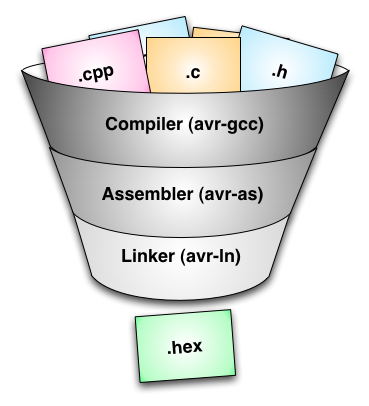
\includegraphics[width=0.26\textwidth]{avr}
\caption{Overview of the AVR toolchain}
\label{fig:tool}
\end{figure}
\paragraph{GCC:} AVR uses the open source GNU Compiler Collection (GCC) with AVR microcontroller as target system. This version of GCC is known as 'AVR GCC' \defcitealias{AVR}{AVR-Libc User Manual, 2008}\citepalias{AVR}. GCC differs from other compilers, it only focuses on translating high level language to target assembly. For AVR GCC there are 3 language options: C, C++ and Ada. 
\paragraph{GNU Binutils: }The next step is done by another open source project called GNU Binutils. This contains the GNU assembler and GNU linker.
\paragraph{AVR-libc:} GCC and Binutils provide the tools to make the machine code but one critical component they do not provide is the Standard C Library. The open source AVR toolchain therefore comes with its own open source C Library project which contains many of the same functions found in the regular Standard C Library. It also adds many additional library functions that are specific to  AVR microcontrollers.
\paragraph{GNU Make:} Finally all pieces must be tied together. This is done by Make, which interprets and executes the Makefile of the project.
%------------------------------
\subsubsection{Memory Sections}
\label{memory}
The available non-volatile memory sections are the \textbf{.text} section (FLASH), which contains the actual machine instructions and the \textbf{.eeprom} section. Many AVR devices have a minimal amount of RAM. This limited amount of runtime memory needs to be shared between the following memory sections:
\begin{enumerate}
\item Initialized variables and static data such as\\ \verb+char message[] = "An error message"+ are stored in \textbf{.data variables}
\item Uninitialized global or static variables: \textbf{.bss variables}
\item Dynamic memory: \textbf{heap}
\item Area used for calling subroutines and storing local variables: \textbf{stack}
\end{enumerate}
The standard RAM layout is shown in figure \ref{fig:RAM}. Since there is no hardware supported memory management, separate regians can overwrite each ohter. Heap and stack can collide if either of them require large memory space or even when the allocations aren't high at all but because heap allocations get fragmented over time and new request don't fit in freed areas.
\begin{figure}[ht]
\centering
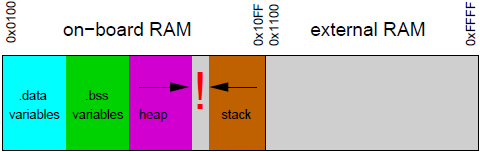
\includegraphics[width=0.48\textwidth]{ram}
\caption{AVR / ATmega1281 standard RAM layout}
\label{fig:RAM}
\end{figure}\\
As discussed in section \ref{memory} the ATmega1281 is uses a modified Harvard architecture, meaning that data can also be stored in program memory space. This is useful when you have constant data and you're running out of room to store it. Remember that many AVRs have limit amount of RAM to store data, but may have available FLASH space left. For the compiler this is however a challenge, which is exacerbated by the fact that the C Language was designed for Von Neumann architectures. So the AVR compiler has to use other means to operate with these separate address spaces (cf. pointer usage). The AVR toolset used the GCC \verb+__attribute__+ keyword, which is used to attach different attributes to function declarations and variables. AVR GCC provides a special attribute called \verb+progmem+ for data declarations and tells the compiler to store the data in Program Memory. To increase the convenience to the end user AVR-libc provides a simple macro \verb+PROGMEM+ which can be found in 'avr/pgmspace.h'. To read the data another macro is provided, which generates the correct address to retrieve the data from Program Memory. Storing data in Program Space incurs extra overhead in terms of instructions and execution time, but usually this is minimal compared to the space savings.\\
\subsubsection{Memory problems}
Libelium's Programming Style Guide warns its users about the amount of memory \verb+USB.print("Test message!")+ requires. The program memory increases due to the instructions and arguments (the chars) needed to print the string, since the message needs to be put in RAM memory first also there precious memory is lost (see the assembly extract in appendix ??).\\
Libelium recommends to do the following:
\usestyle{vs} %other useful styles are, bw,  borland, vs
% Include the source code 
\includecode{mem1.cpp}
This however still uses both program and data memory and is only useful if one wants to print the same message in different parts of the program, so this is not really a solution. The only way to save RAM memory while printing messages is to hard code them into the heap by doing the following:
\usestyle{vs} %other useful styles are, bw,  borland, vs
% Include the source code 
\includecode{mem2.cpp}
A less cumbersome way would be to give the message and an address where to store the message as argument of a recursive matrix which does this operation for us. However, standard C Language macro's cannot simply split a string into characters. So the only ways to save RAM is to hard code the string as data or to store the string in Program Space and use the \verb+strcpy_P+ to copy the string to stack when it is needed. 
\subsection{Libelium IDE and API}
\subsubsection{Waspmote-IDE}
The Libelium IDE offers some advantages compared to using other IDE's. For example by using Eclipse it is possible to update programs that are to big ( > 120KB ), over-writing the bootloader. Then they must be sent back to Libelium to restore them. The Waspmote IDE does not allow this accident, so Libelium does not support using other IDE's in an official way so that there is no valid warranty if you've erased the bootloader. Their IDE is far from perfect however, some issues we've experienced are:\\
\begin{itemize}
\item Opening a second or more instance of the IDE sometimes re-opens the previously active files, making it confusing to detect which one you were working in so you end up with two unsaved versions of the same code.
\item Once you start compiling (which takes a lot of time) there's no way to stop it, the stop button does not work.
\item Uploading immediately after compiling will first re-compile it anyway.
\item There is no complete C/C++ support. For example using simple enums is not possible. A workaround is to place the code in additional .h or .cpp files.
\item Auto-completion for the Libelium API functionality would be a great addition.
\end{itemize}
\bigskip
Also the Waspmote's (V1.1) hardware slows down the programming process:
\begin{itemize}
\item Uploading the code takes a lot of time: 1.5 - 2 minutes.
\item The uploading process fails if:
\begin{itemize}
\item The XBee is present
\item The hibernate jumper is not present when the mote is in hibernate
\item The little power switch has been turned off
\end{itemize}
\end{itemize}
Often you will want to turn off the power switch temporarily to analyse the content of the serial monitor. Especially in pair programming there is often one requirement you forget and the Waspmote does not check for this on beforehand. It will first compile and do as if it is uploading your code, disappointing you at the end of the process.\\
When debugging bigger program these actions come even more annoying. Suppose you are testing a program which measures sensors, sends the values and hibernates. Then you must:
\begin{enumerate}
\item Remove the sensor board
\item Place the hibernate jumper
\item Remove the XBee
\item Upload
\item Place the XBee
\item Remove the hibernate jumper
\item Re-mount the sensor board
\end{enumerate}
And this is not the end of the list. Removing the hibernate jumper causes the Waspmote to crash one out of two times. Resetting the mote has no effect in this case, just keep inserting and removing the little jumper until it agrees with what you want.
%------------------------------------
\subsubsection{Waspmote-API}
\label{LibAPI}
To facilitate the programming Libelium offers a quite big API and after some exploring you are quickly started with it. The structure of the API is very simple, there is little to no inheritance. In this section, the most important classes are indicated with a red box and are recommended to explore before starting future programming.
\paragraph{Original structure}
Each module or concept has its own class, for example all RTC functions are in 'WaspRTC.h' and 'WaspRTC.cpp'. To be able to use those functions in the IDE an object from the class 'WaspRTC' must be created. This object is created by default by the library and it is public to all libraries. All types to be run on the API can be found in the 'WaspClasses.h' file and each file also includes this file so it is aware of all available types. Please see appendix \ref{appendixC} for a complete overview.\\
For our application WaspXBeeZB is one of the most important classes. It inherits from WaspXBee Core and this way it is also related to the WaspXBee class. Figure \ref{fig:API2} displays the relationship with the AVR-libc libraries and the Waspmote hardware. For example \verb+typedef unsigned char uint8_t+ can be found in 'stdint.h'.\\ 
\begin{figure*}[ht]
\centering
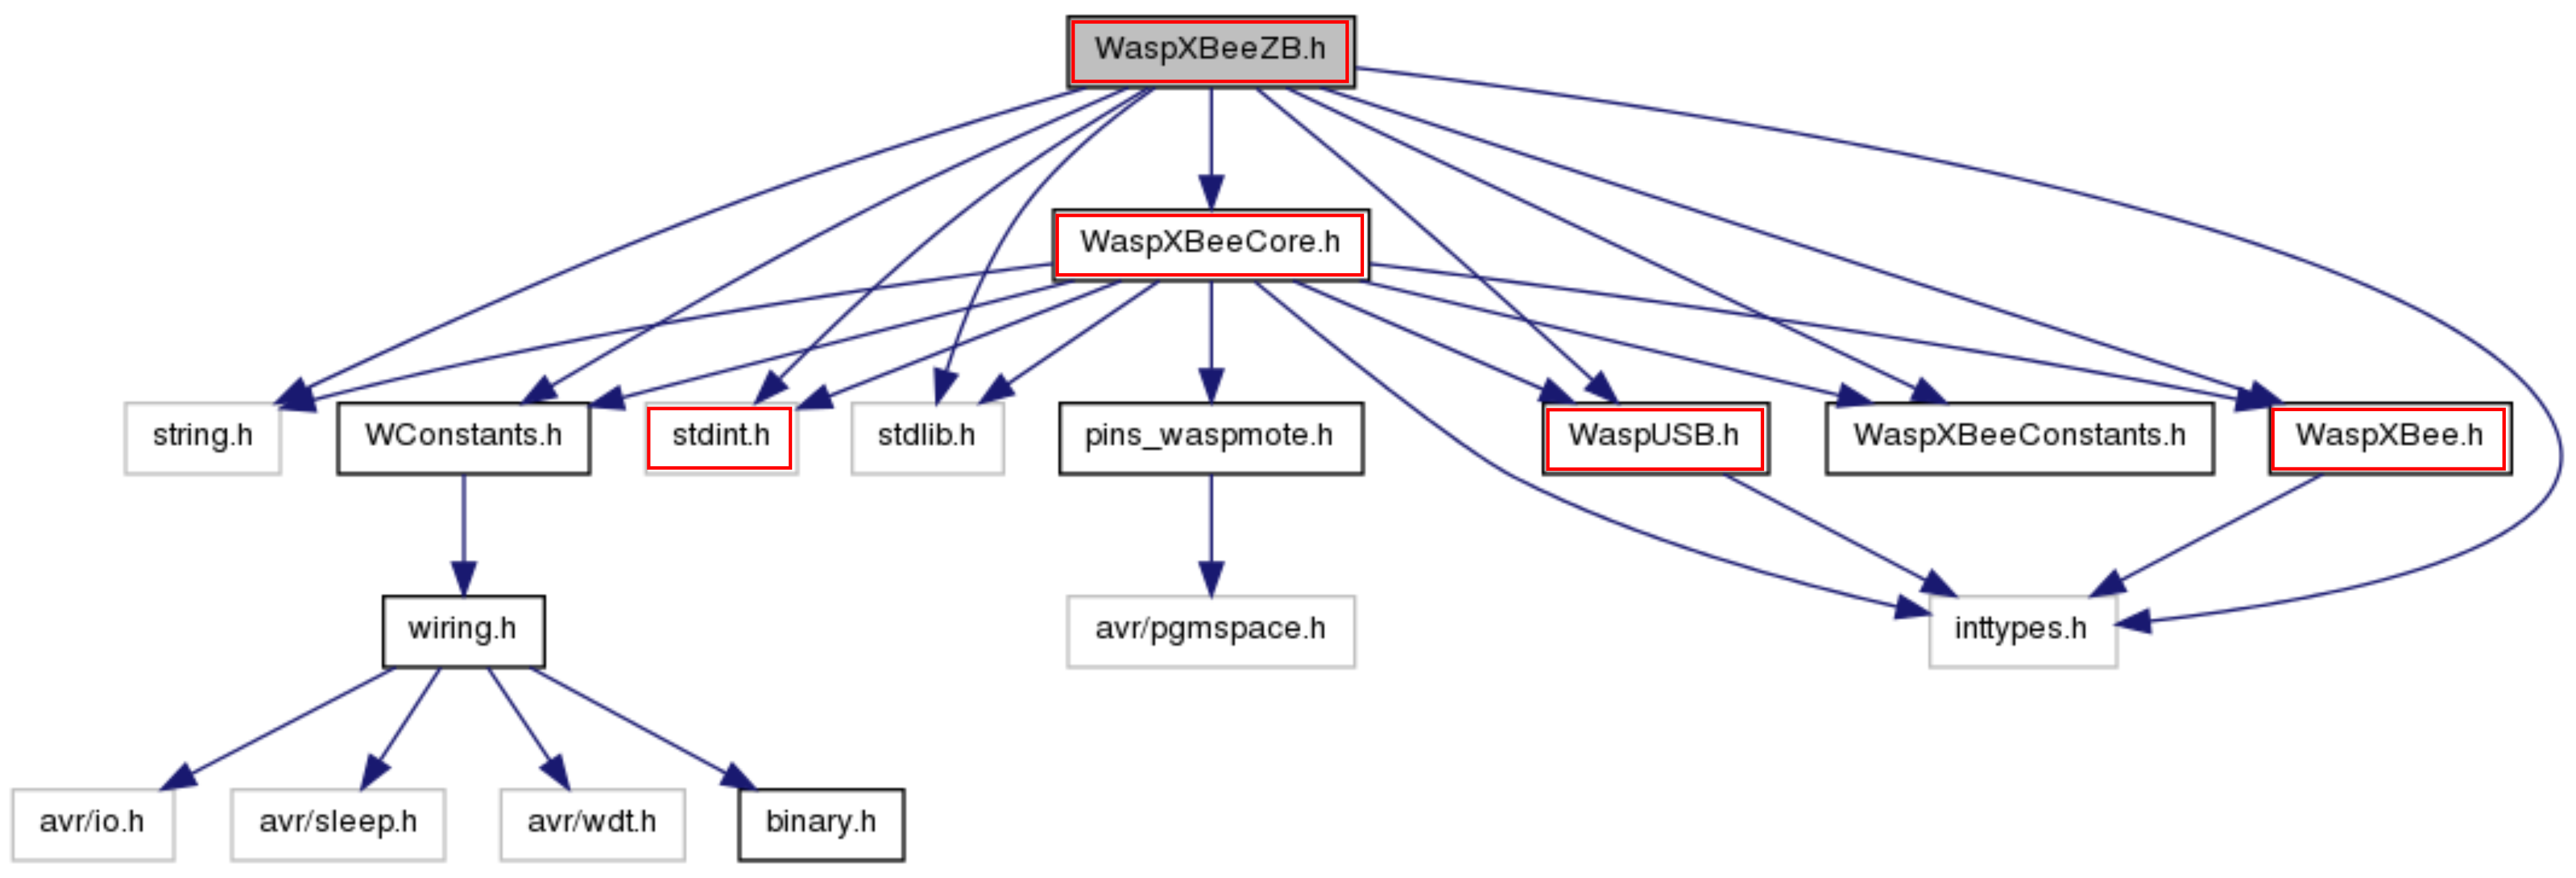
\includegraphics[width=0.98\textwidth]{API2}
\caption{Reduced dependency of Waspmote core libraries}
\label{fig:API2}
\end{figure*}
\noindent During the development of our program the Waspmote showed several strange effects that could only be explained by bad stack management or heap and stack conflicts. Because of this lack of free memory (SRAM, 8KB) we discovered that the V1.1 API wastes a lot of memory by always including all libraries despite not using them. As a fix Libelium recommends to remove all classes you do not use, and there fields that are used in other classes, 'just' going through the compiler errors one by one. After this our program had enough free memory and showed normal behaviour.
%------------------------------------
\paragraph{Added functionality}
To facilitate programming extra functionality has been added to the Libelium API. They are inside files containing the original name with the 'Utils' addition, for example 'WaspRTCUtils.h' and can be found in 'BjornClasses.h'.
%----------------------------------------------------------------  




%----------------------------------------------------------------------------------------
\subsection{Sleep options}
After default configuration the Waspmote will send only its battery level to the default gateway, check for received commands and go into hibernate mode for 1 minute. In a first approach, which focusses on longer battery life, ZigBee sleep options are not taken into account. With ZigBee sleep enabled, routers and coordinators can buffer incoming RF data for their end device children. However, they can only do this up to 30 seconds \defcitealias{XBEE}{XBee/XBee-Pro ZB RF Modules User Manual, 2012}\citepalias{XBEE}. When an end device sleeps longer than 30 seconds, they should send a transmission when they wake to inform other devices that they are awake and can receive data. This is exactly what the first approach does, except it completely disconnects the XBee and sleep intervals are much longer.\\
To make the web service more reactive, this latency has been removed in the second approach. Here XBee sleep is enabled and end devices will respond to commands within 30 seconds.
In a last approach we have a look at how the energy usage of the first approach can be optimized even more.  
\subsubsection{Without ZigBee sleep}
This section discusses algorithms which can be used to measure sensors at variable times. It supposes the Waspmote uses either \textit{Hibernate} or \textit{Sleep} mode, completely disconnecting the XBee. Since it is not possible to combine RTC for both hibernate and sleep mode, a tweak has been implemented to use the Watchdog instead. This way the program can automatically chose which sleep mode to invoke, depending on the next duration to sleep. In hibernation mode the node is completely disconnected from the main battery and the program stops. This makes that all variables lose their values and must be stored in EEPROM memory. Each of the next techniques present with benefits and drawbacks and since we are working with embedded systems with limited possibilities, one should also consider to limit the users options to facilitate the calculations.
\paragraph{Calculate only the next time to sleep}
Each algorithm will have to store the individual sleep times per sensor. To support this algorithm also a copy of the original time will be saved and each time the node wakes up it will look for the smallest next time to sleep. This number will be subtracted from the other sleep times in the array. When a value becomes zero it will be restored with its original value and the cycle continues.  For an example which demonstrates this process please see appendix \ref{AppendixC}.\\
This process is fast and simple. However, the main advantage is that the node has to write to EEPROM each time it wakes up. According to the Atmel datasheet, the EEPROM of the ATmega1281 has an endurance of at least 100,000 write / erase cycles. The following equation indicates the problem for an interval of 10 seconds:
\begin{equation}
\frac{100000 \mathrm{writes} \cdot 10 \mathrm{s}}{60 \mathrm{s} \cdot 60 \mathrm{min} \cdot 24 \mathrm{h}}= 11,57 \: \mathrm{days} 
\label{eq:1}
\end{equation}
But the processors has 4Kbytes EEPROM on board so we don't have to write to the same place every time. Since EEPROM is written on a 'per cell' basis this can extend the lifetime. Our sensor mask can contain up to 16 values of 2 bytes. This leads to the next result:
\begin{equation}
\frac{100000 \mathrm{writes} \cdot 10 \mathrm{s} \cdot 4\mathrm{KB}}{60 \mathrm{s} \cdot 60 \mathrm{min} \cdot 24 \mathrm{h} \cdot 365\mathrm{days} \cdot 32\mathrm{B}} = 3,96\: \mathrm{years}
\end{equation}
We still must store where the data is stored but this won't cause big problems since we only have to rewrite this cell 125 times:
\begin{equation}
\frac{4\mathrm{KB}}{32\mathrm{B}} = 125 \: \mathrm{writes}
\end{equation}
\paragraph{Calculate all next times to sleep}
Another possibility is calculate as much as possible or maybe even all sleep necessary times. This algorithm first calculates the least common divider of the given measuring intervals. Afterwards memory is allocated to store the multiples of the values. When the LCM divided by the smallest measuring interval is smaller than the size of the allocated space, all values can be stored in EEPROM. If this is not the case also the last multiplier of the measuring interval must be stored, so when the last value is reached, the next series can be calculated.\\
Each time the Waspmote wakes up, it will compare its current RTC value with the times stored in EEPROM. The biggest stored time that is an integer multiple of the RTC value is the current position in the array. With this time the sensors to measure and the next time to sleep can be determined.
\paragraph{Limit user control}
Depending on the next time to sleep the program could decide for itself to go into hibernate, deepsleep or sleep with XBee sleep mode. Also, when the program detects inefficient measuring intervals, for example, 1 minute and 2 minutes 10 seconds, this can be notified to the installer or even be refused during setup.
%----------------------------
\subsubsection{With ZigBee sleep}
... ...
\subsection{Program Structure}
\subsubsection{Sending and Receiving}
In the API of Waspmote v1.1 Libelium uses an 'Application Header' which is shown in figure \ref{fig:appH} to send and receive data. This header takes care of packet fragmentation if packets exceed the maximum payload limit and can also be used by the receiver to treat the packet or fragment. The header itself is sent inside the RF Data field of the API Frame Structure.\\
\begin{figure}[ht]
\centering
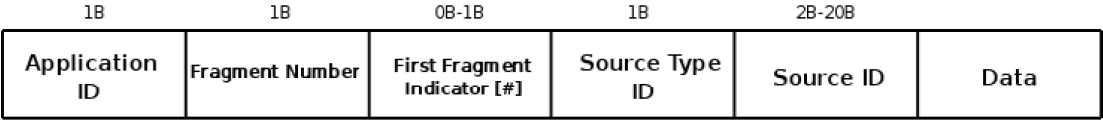
\includegraphics[width=0.48\textwidth]{appHeader}
\caption{Application Header}
\label{fig:appH}
\end{figure}
The Waspmote and gateway programs use the 'Application ID' field in this header to distinguish different data in sent packets. In a first approach this extra layer we developed also serves as acknowledgement in the communication protocol. Depending on the 'Application ID' the layer contains a sensor mask is (a 16 bit-flag) and data. Examples are 'ADD\_NODE\_REQ' and 'CH\_SENS\_FREQ\_REQ'. Appendix \ref{AppendixG} shows a complete overview off all options.\\
To easily switch between the different requests and select the sensors contained in the received mask the program uses static function pointers. An example is given below:
\usestyle{vs} %other useful styles are, bw,  borland, vs
% Include the source code 
\includecode{fp.cpp}

\subsubsection{Without ZigBee sleep mode}
In this mode there is no difference between routers and end devices on XBee level. The only difference in program execution is that the sleeping period is skipped for routers. The user can set the device role during setup or even later on by sending a command to the Waspmote, which makes it easy to change a mote's device role. The device role is stored in the xbeeZB device type identifier (see \defcitealias{ZBGUIDE}{Waspmote ZigBee Networking Guide, 2012}\citepalias{ZBGUIDE} and '\textbf{WaspXBeeZBNode.h}').
To better understand the next sections please have a quick look at the program flow chart in figure \ref{fig:flow}.
\paragraph{Device start-up}
Whether we come out of a hardware reset or a hibernate reset, the first thing the node will do is try to establish a connection with the network. Depending which reset we come from different routines will be executed. In normal operation mode this process only takes about 2 seconds (Please see appendix \ref{fig:envA} for more measurement results). However, when a node is not able to join a network it will go into panic mode. This means that if the operating sleeping time is small, this time will be ignored and the node will wake up less frequently until it is able to rejoin the network, that way saving battery power. Supposing the node is able to rejoin the network, it will send the number of panics it experienced to the coordinator so a network administrator can investigate of the severity of the problem.

\paragraph{Full initialization}
When the program is executed for the first time or when a hardware reset is detected the XBee will execute a full initialization process and the RTC will be set to zero. This means the default PAN ID and possibly other user settings like node ID will be written to the XBee. After this write the XBee must be re-setted (turn the power off and back on) and only than the joining attempts can start. This means full initialization takes about 9 seconds on average. 

\paragraph{Reduced initialization}
By not resetting the PAN ID but fetching it from the XBee's memory the joining process only takes about two seconds. Unfortunately a disadvantage of this shortened setup is that the XBee is no longer able to detect if the coordinator or his parent is actually available. The program will only notices this for the first time when it is trying to send a message. If this function results in a send error the program will do a full setup routine and resend the message. If the node then fails again to send the message we can conclude that the coordinator is really off-line or that there are no joinable nodes within range. 


\paragraph{Measuring sensors}
sensor float to bytes conversion... ...
\paragraph{Sending samples}
escaping zeros... ...
app ID = 10: 'IO\_DATA'... ...
see appendix ?? for all our packets... ...
